\documentclass[10pt]{article}
\usepackage{ngerman}
\usepackage[utf8]{inputenc}
\usepackage{graphicx}
\usepackage{subcaption}
\usepackage{hyperref}
\title{\textbf{Hürth-blüht Jahresbericht 2020}}
\author{Ivo Bathke\\
		BUND Hürth\\}
\date{}
\begin{document}

\maketitle

\begin{figure}[h!]
  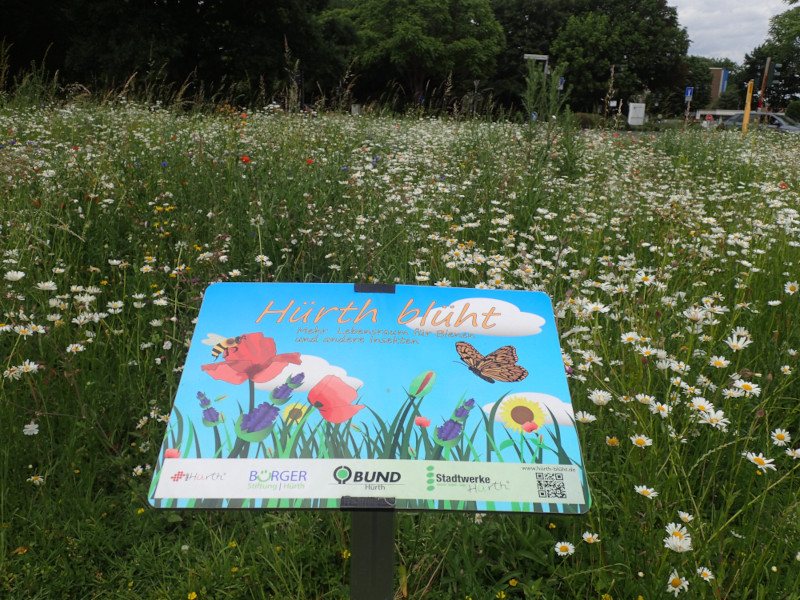
\includegraphics[width=\linewidth]{img/titel.jpg}
\end{figure}

\newpage

\section{Einführung}
Im nun zweiten Jahr von \textbf{Hürth-blüht} wollen wir die Entwicklung der Flächen betrachten und auch 4 neue Flächen vorstellen, die in 2020 angelegt wurden.


Im Frühjahr wurde bei einem Treffen von BUND, Stadt Hürth und Stadtwerken das Projekt besprochen und das Jahr geplant. Dabei wurden neue Flächen beschloßen und ausgesucht sowie die Vorgehensweise besprochen.
Es wurde u.a. eine Streifenmahd beschloßen, wobei bei der Mahd eine Streifen stehen gelassen wird, um Insekten weiterhin Nahrung und Deckung zu bieten.

Das Projekt \textbf{Hürth-blüht} wurde zum Bundeswettbewerb "`Naturstadt"' eingereicht, war jedoch leider nicht erfolgreich. Es wurden insgesamt 322 Projektideen eingereicht, wovon nur 40 Beiträge ausgewählt wurden.

Die zunehmend trockenen Sommer sind auch für die Blühflächen eine Herausforderung. Insgesamt kommen die Flächen aber gut damit zurecht, deutlich besser als kurzgemähten Wiesen.
Es gibt jedoch auch Probleme an besonders trockenen Standorten, wie etwa dem Hürther Bogen.

Die Resonanzen aus der Bevölkerung waren durchaus positiv. So wurde häufig beobachtet wie Selfies vor den Blühflächen gemacht wurden, auch wurden Blumensträuße für Oma gepflückt und manche Passanten wähnten sich bereits im Urlaub.

Die Blühflächen haben neben der Optik aber auch noch noch einen weiteren Grund: Dem Insektensterben und dem Verlust an Artenvielfalt entegegen zu treten. Die botanische Vielfalt konnte allein schon durch die Blühwiesen erhöht werden. Die Flächen wurden auch durch etliche Insekten angenomen, deutlich mehr als in den umliegenden gemähten Flächen. Jedoch meistens eher häufige Arten, vermisst werden weiterhin z.B.: Blutströpfchen, Dickkopffalter und Große Heupferde.


\newpage

\section{Burgpark}

\begin{figure}[h!]
  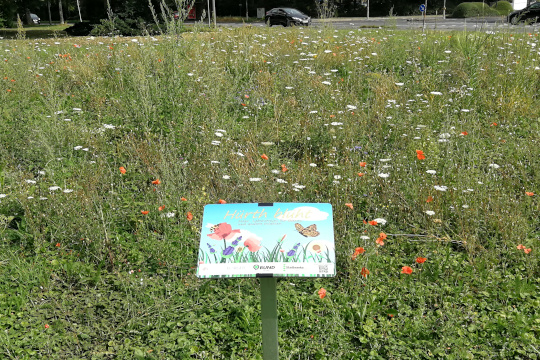
\includegraphics[width=\linewidth]{img/infotafeln.jpg}
  \caption{Burgpark}
  \label{fig:boat1}
\end{figure}

\begin{flushleft}
Zustand der Fläche ist sehr gut.

Der Effekt der Streifenmahd konnte hier gut beobachet werden.
So waren im stehen gelassenen Teil weiterhin viele Insekten zu sehen, während im gemähten Teil die nächsten Pflanzenarten hochwuchsen.

Der neue Fahrradweg wird vermutl. einen Teil abschneiden. 
Dies sollte am anderen Ende der Fläche wieder angefügt werden.


\begin{figure}[h!]
  \centering
  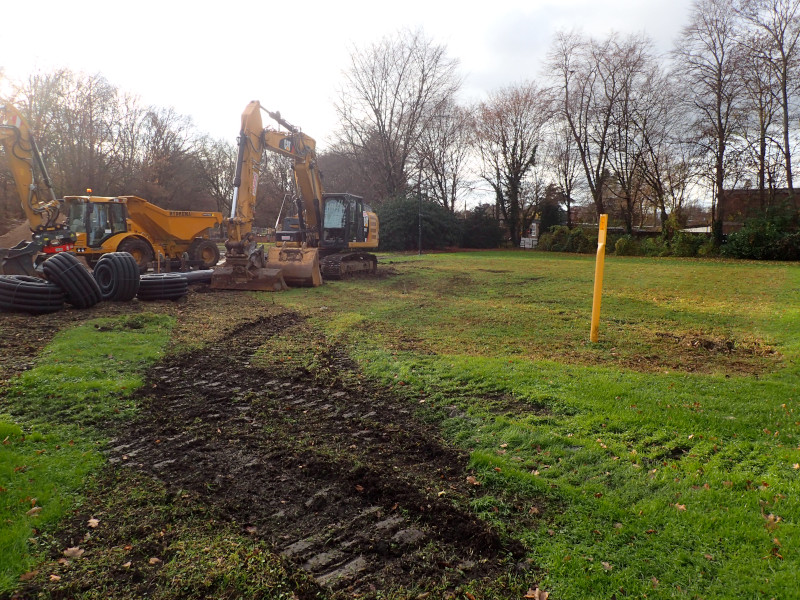
\includegraphics[width=0.45\linewidth]{img/burgpark/baustelle.jpg}
  \caption{Baustelle an und auf Blühfläche}
  \label{fig:boat1}
\end{figure}

\end{flushleft}

\newpage

\textbf{Insekten im Burgpark:}

\begin{figure}[h!]
  \centering
  \begin{subfigure}[b]{0.41\linewidth}
    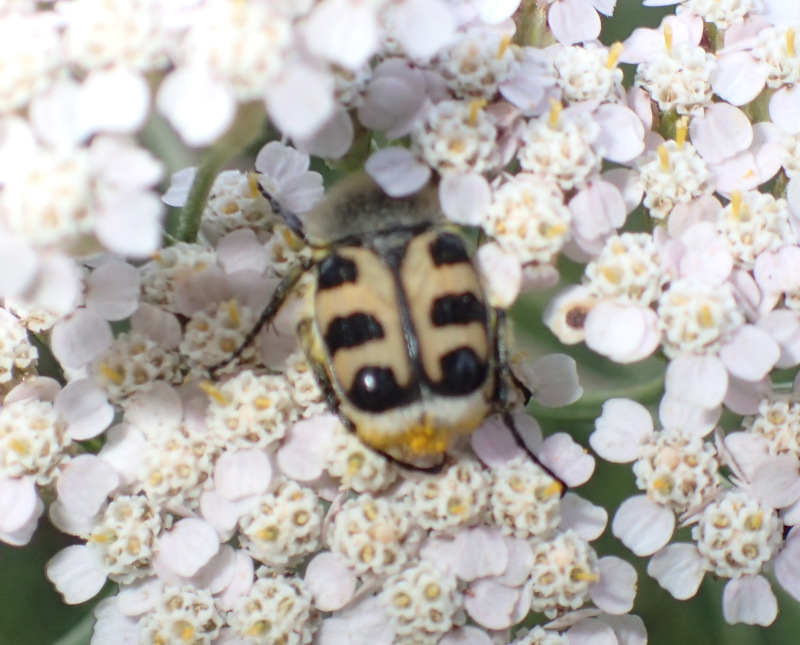
\includegraphics[width=\linewidth]{img/pinselkaefer.jpg}
    \caption{Pinselkäfer}
  \end{subfigure}
  \begin{subfigure}[b]{0.50\linewidth}
    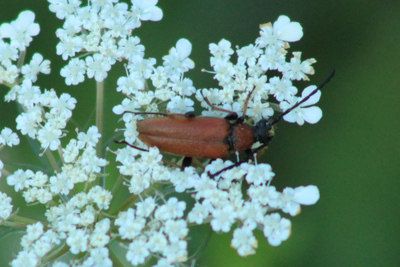
\includegraphics[width=\linewidth]{img/schmalbock.jpg}
    \caption{Rothalsbock}
  \end{subfigure}
  \begin{subfigure}[b]{0.48\linewidth}
    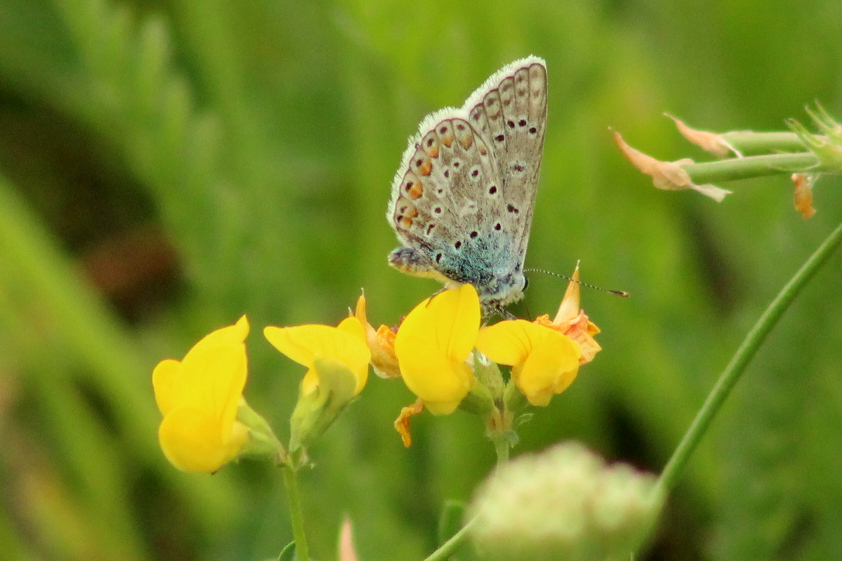
\includegraphics[width=\linewidth]{img/blaeuling.jpg}
    \caption{Hauhechel-Bläuling}
  \end{subfigure}
  \begin{subfigure}[b]{0.43\linewidth}
    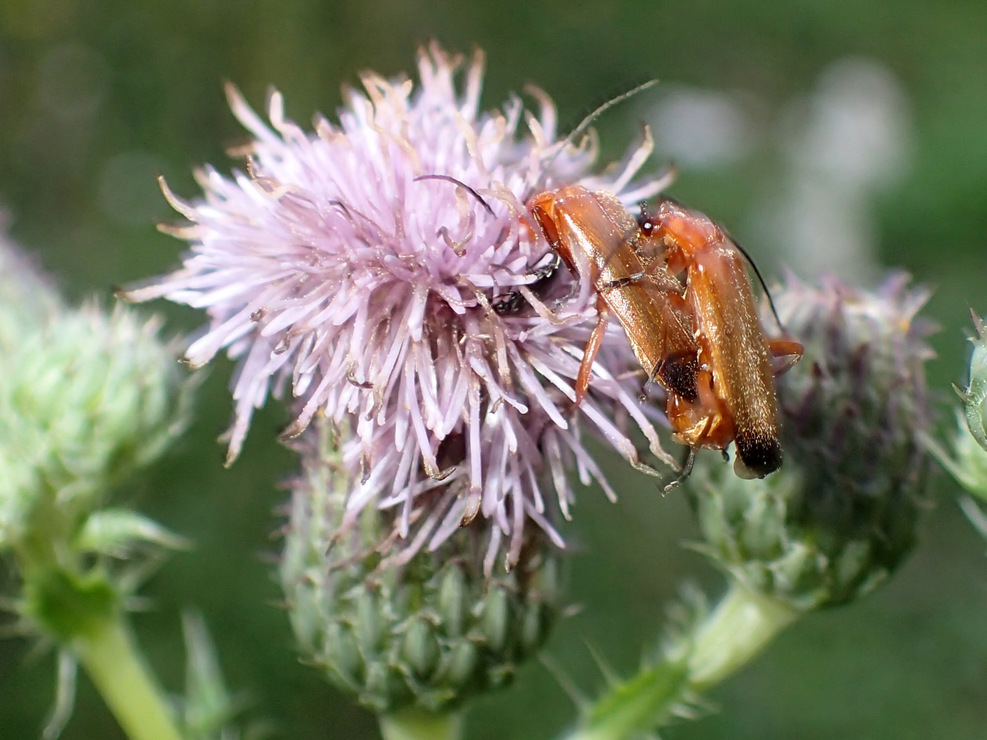
\includegraphics[width=\linewidth]{img/weichkaefer.jpg}
    \caption{Ockerbrauner Weichkäfer}
  \end{subfigure}
  \caption{Insekten Burgpark}
\end{figure}

Auf der Blühfläche im Burpark konnten viele, blütenbesuchende Insekten beobachtet werden.

\newpage
\section{Gesamtschule}
\begin{figure}[h!]
  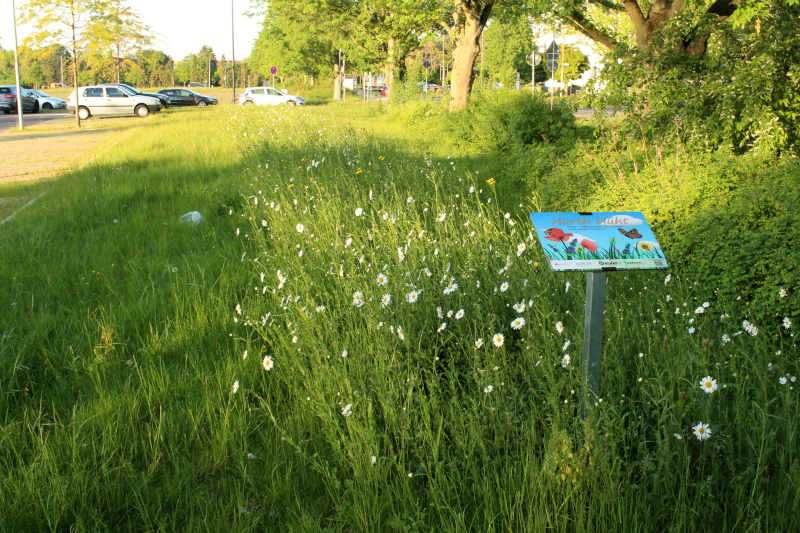
\includegraphics[width=\linewidth]{img/gesamtschule/mai.jpg}
  \caption{Gesamtschule}
  \label{fig:boat1}
\end{figure}

Nach einem eher mageren Start in 2019 ist die Fläche 2020 sehr gut angegangen.

Hier wäre die Überlegung auch auf den Grünflächen des Parkplatz Blühflächen anzulegen.

Ein Highlight war eine auf Grashüpfer lauernde Wespenspinne im Spätsommer, im stehengelassen Teil.


\begin{figure}[h!]
  \centering
  \begin{subfigure}[b]{0.34\linewidth}
    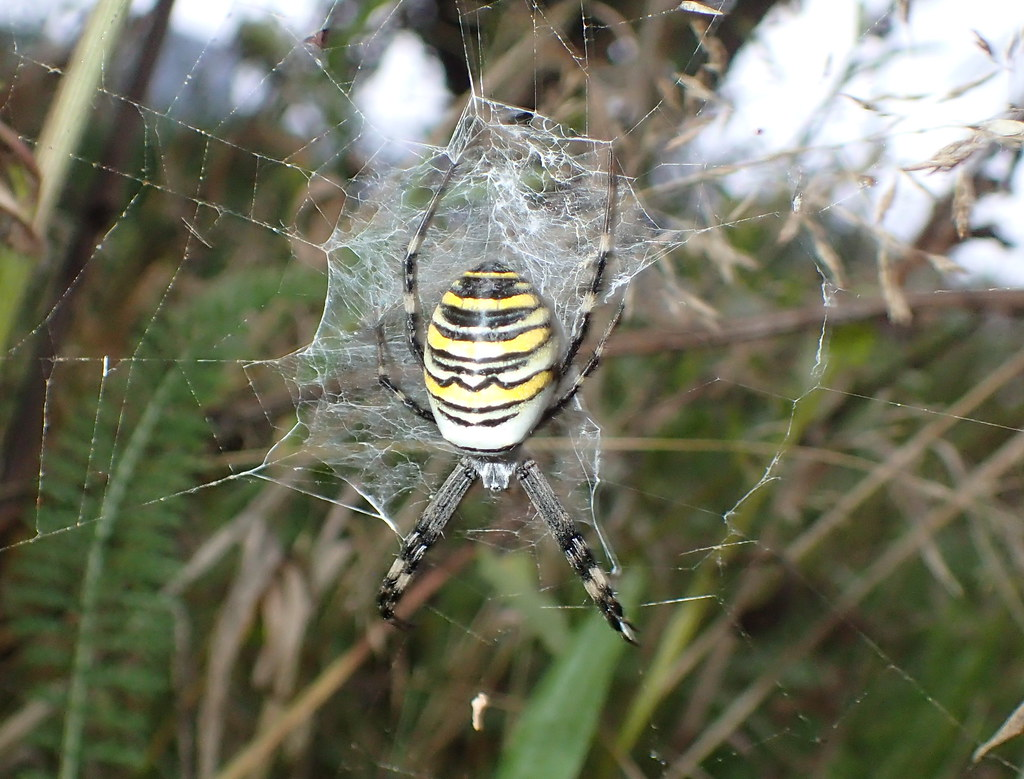
\includegraphics[width=\linewidth]{img/gesamtschule/wespenspinne.jpg}
    \caption{Wespenspinne}
  \end{subfigure}
  \begin{subfigure}[b]{0.38\linewidth}
    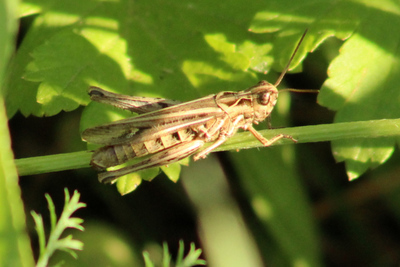
\includegraphics[width=\linewidth]{img/gesamtschule/grashuepfer.jpg}
    \caption{Feld-Grashüpfer}
  \end{subfigure}
  \caption{Insekten Gesamtschule}
\end{figure}

\clearpage
\section{Sudetenstr.}
\begin{figure}[h!]
  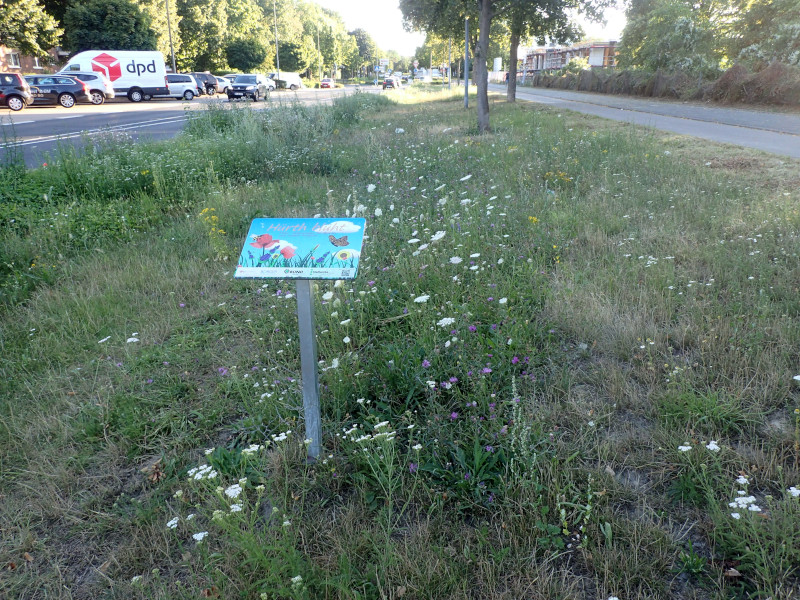
\includegraphics[width=\linewidth]{img/asg/juli.jpg}
  \caption{Sudetenstr. 21. Juli 2020}
\end{figure}
Der Blühstreifen wurde versehentlich im April gemäht, daher gab es hier einen etwas schwierigen Start und eine magere Margeriten-Phase.

Im weiteren Verlauf hat die Fläche aber gut aufgeholt, trotz der Trockenheit. 
Es gibt jedoch ein paar sehr trockenen Störstellen, insgesamt aber kein Grund zur Sorge. 

Im August stand auch die umgebene Fläche recht hoch. Hier wäre zu überlegen ob statt des geschwungenen Blühstreifen die gesamte Fläche als Blühstreifen behandelt werden sollte.

\clearpage
\section{Frechenerstr.}
\begin{figure}[h!]
  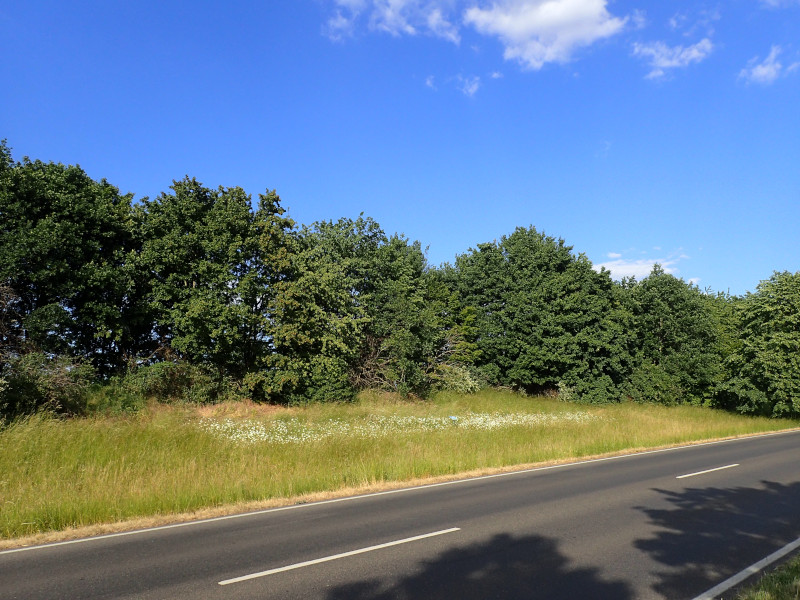
\includegraphics[width=\linewidth]{img/frechenerstr/mai.jpg}
  \caption{Frechenerstr. 29. Mai 2020}
\end{figure}

Der Blühstreifen an sich ist gut entwickelt, geht jedoch etwas unter in der größeren umgebenen hochstehenden Wiese.

Hier wäre es gut wenn die gesamte Fläche sich zur Blühfläche entwickelt. Der Mahdplan müßte dann entsprechend angepasst werden.

\clearpage
\section{Sielsdorf}
\begin{figure}[h!]
  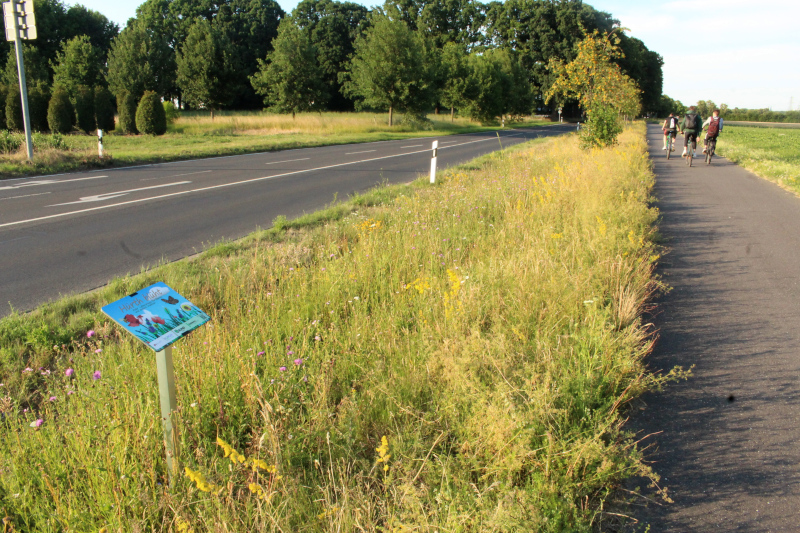
\includegraphics[width=\linewidth]{img/sielsdorf/juni.jpg}
  \caption{Sielsdorf 24. Juni 2020}
  \label{fig:sielsdorf}
\end{figure}

Der Blühstreifen zwischen Fahrradweg und Straße ist gut entwickelt und blüht sehr vielfältig.

\clearpage
\section{Heristalstr.}
\begin{figure}[h!]
  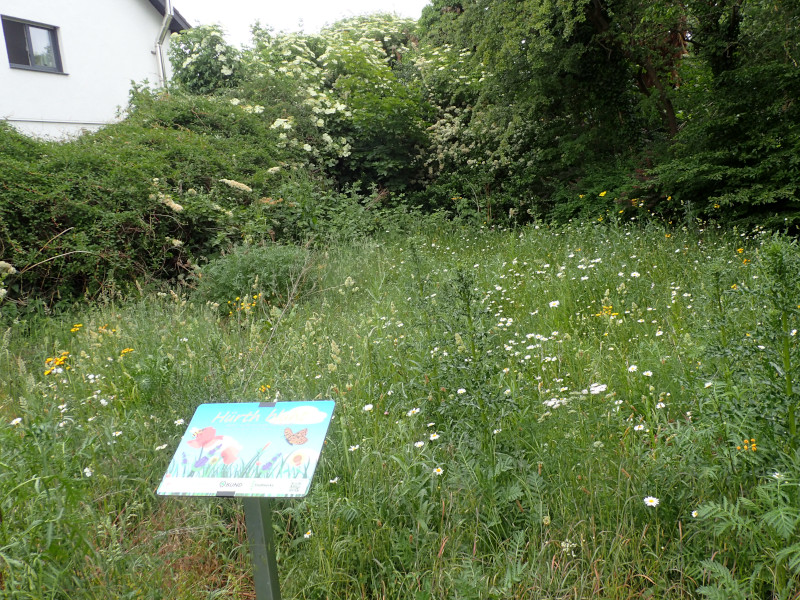
\includegraphics[width=\linewidth]{img/heristal/mai.jpg}
  \caption{Heristalstr. 22. Mai 2020}
  \label{fig:boat1}
\end{figure}

Die Fläche ist klein und etwas schattig und wird bedrängt von Brombeeren aus den umgebenden Hecken.
Dennoch ist sie gut entwickelt. Auffällig ist der viele Rainfarn in der Fläche.

Hier wurde im Juni komplett gemäht, die Fläche war jedoch bald wieder voll in Blüte.

\clearpage
\section{Randkanal}
\begin{figure}[h!]
  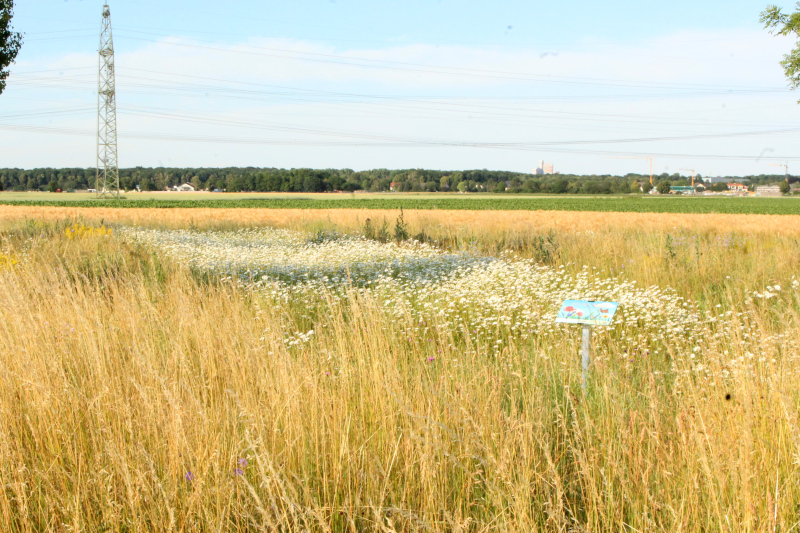
\includegraphics[width=\linewidth]{img/randkanal/juni.jpg}
  \caption{Randkanal 24. Juni 2020}
  \label{fig:randkanal juni}
\end{figure}

Die 2 Blühflächen innerhalb der Kompensationsfläche sind gut entwickelt.

Viele Insekten lassen sich dort beobachten, was sicherlich auch an der Größe der Fläche insgesamt liegt und auch an der unversiegelten Umgebung.

\clearpage
\textbf{Insekten am Randkanal:}

\begin{figure}[h!]
  \centering
  \begin{subfigure}[b]{0.44\linewidth}
    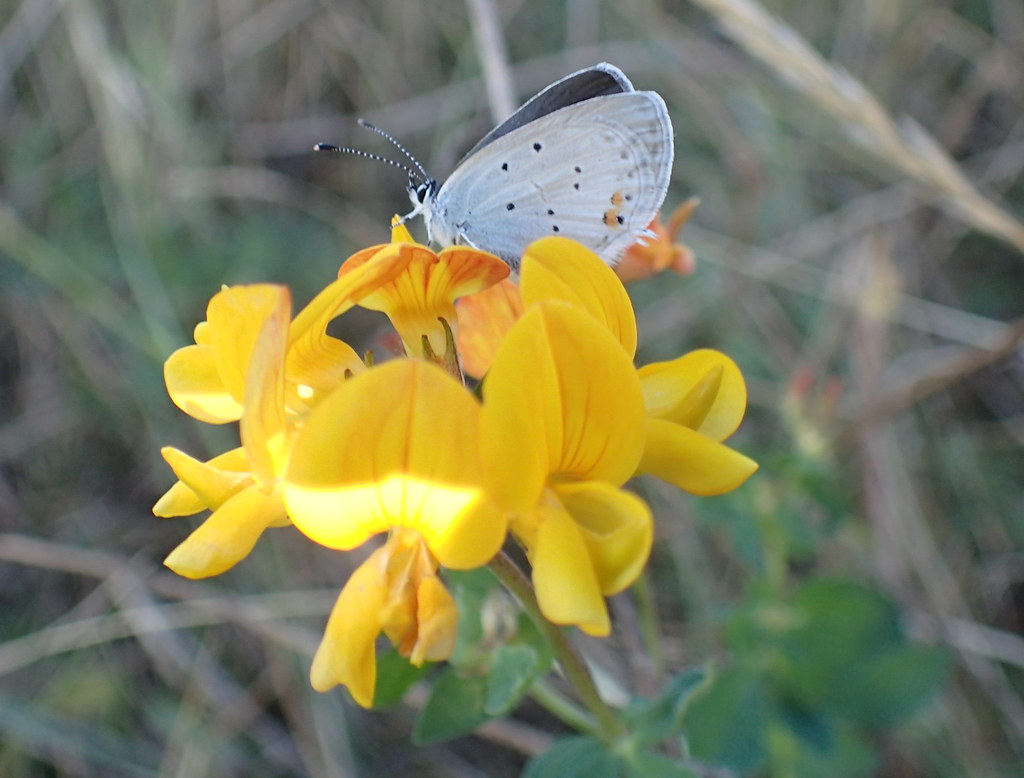
\includegraphics[width=\linewidth]{img/randkanal/blauling.jpg}
    \caption{Kurzschwänziger Bläuling}
  \end{subfigure}
  \begin{subfigure}[b]{0.44\linewidth}
    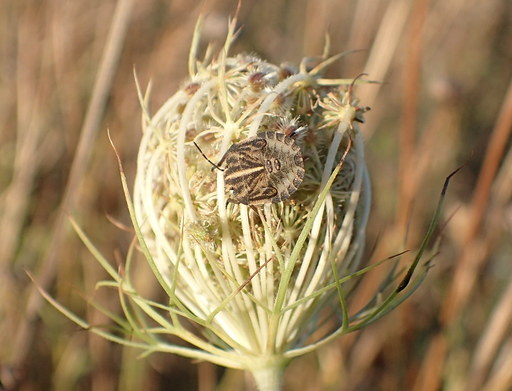
\includegraphics[width=\linewidth]{img/randkanal/streifenwanze.jpg}
    \caption{Larve Streifenwanze}
  \end{subfigure}
  \begin{subfigure}[b]{0.45\linewidth}
    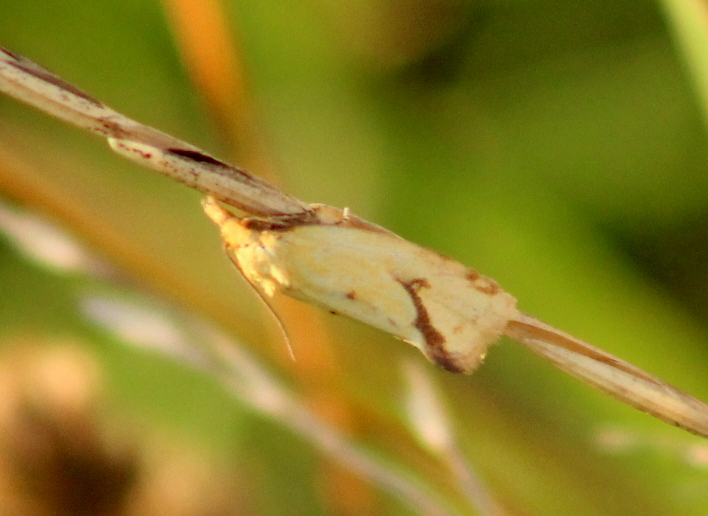
\includegraphics[width=\linewidth]{img/randkanal/distelwickler.jpg}
    \caption{Distelwickler}
  \end{subfigure}
  \begin{subfigure}[b]{0.43\linewidth}
    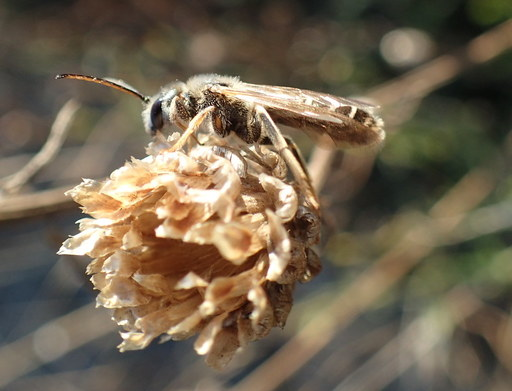
\includegraphics[width=\linewidth]{img/randkanal/wildbiene.jpg}
    \caption{unbest. Wildbiene}
  \end{subfigure}
  \caption{Insekten Randkanal}
\end{figure}

\clearpage
\section{H.Sürthweg}
\begin{figure}[h!]
  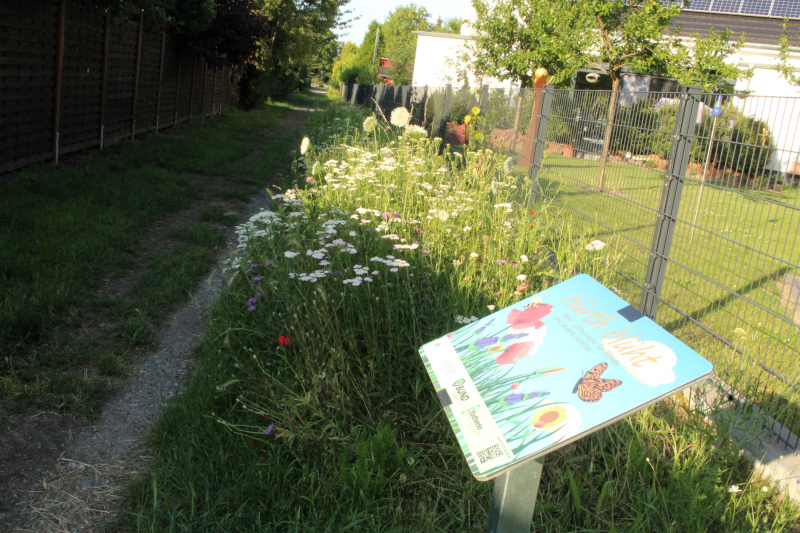
\includegraphics[width=\linewidth]{img/suerthweg/juni.jpg}
  \caption{H.Sürthweg. 24. Juni 2020}
\end{figure}

Auch hier wurde laut Anwohner versehentlich im Frühjahr gemäht.
Die Fläche hat sich später dann gut entwickelt. 

\clearpage
\section{Hürther Bogen}
\begin{figure}[h!]
  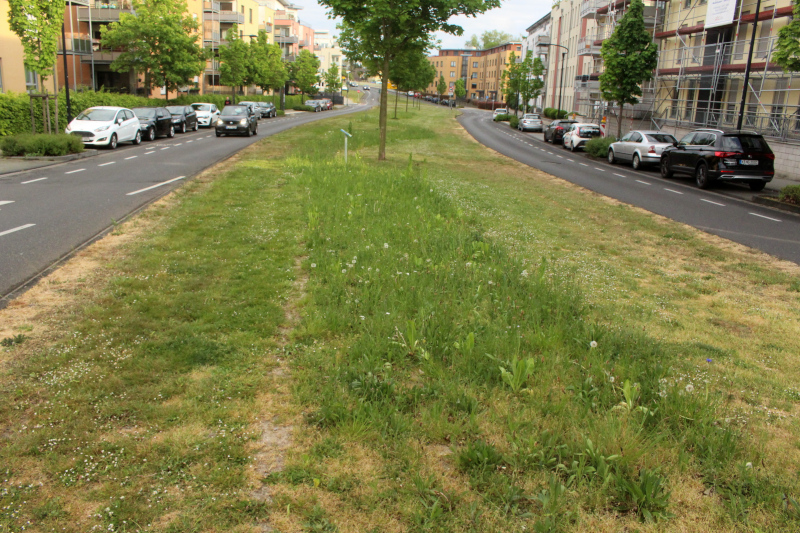
\includegraphics[width=0.95\linewidth]{img/bogen/april.jpg}
  \caption{Hürther Bogen 28. April 2020}
\end{figure}

Die Fläche insgesamt leidet sehr unter der Trockenheit.
Hier ist es besonders trocken, vermutlich wegen der Hanglage und auch durch die Umgebung aus Straßen, Häusern und Beton. Dies führt zu einer weiteren Aufheizung und Verdunstung.

Evtl. sollte hier eine etwas andere Saatmischung verwendet werden, die mit arideren Bedingungen zurecht kommt.

Trotz allem blühte es auch hier und einige Insekten wurden beobachtet. 

\begin{figure}[h!]
  \centering
  \begin{subfigure}[b]{0.45\linewidth}
    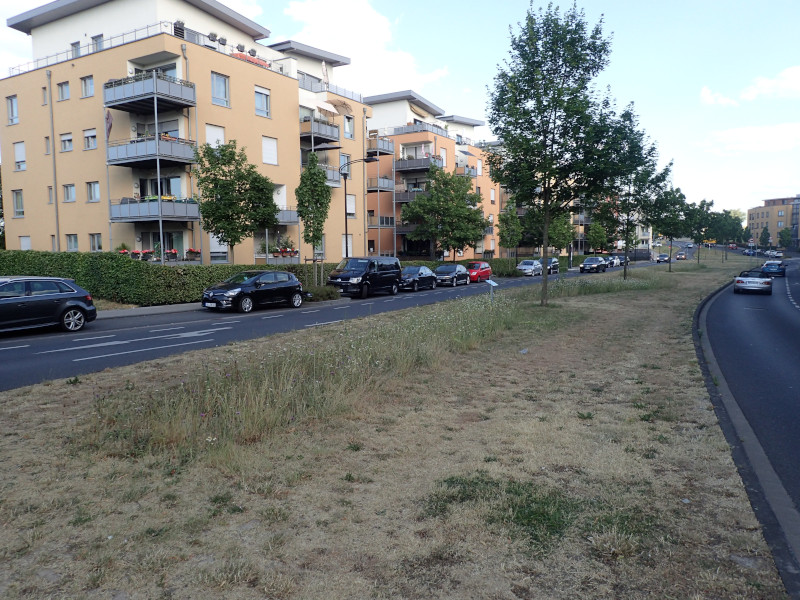
\includegraphics[width=\linewidth]{img/bogen/mai.jpg}
    \caption{trockener Mai}
  \end{subfigure}
  \caption{Hürther Bogen}
\end{figure}


\clearpage
\textbf{Insekten am Hürther Bogen:}

\begin{figure}[h!]
  \centering
  \begin{subfigure}[b]{0.47\linewidth}
    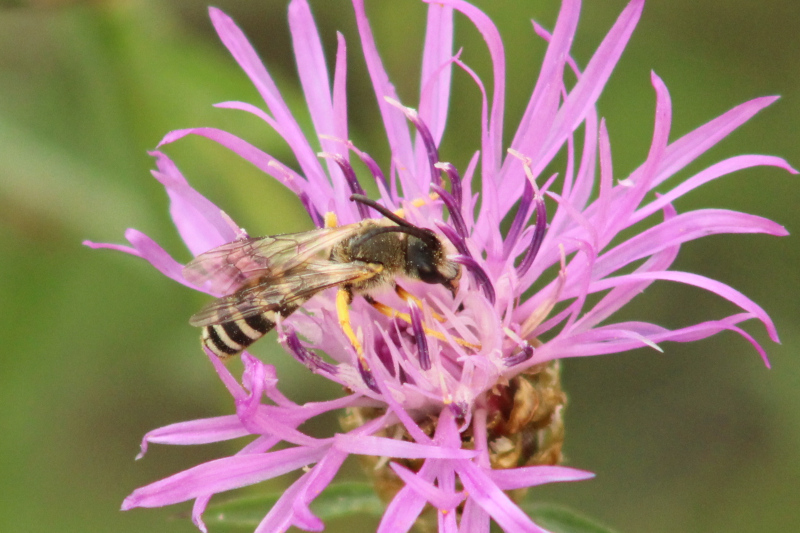
\includegraphics[width=\linewidth]{img/bogen/wildbiene.jpg}
    \caption{Gelbbinden-Furchenbiene}
  \end{subfigure}
  \begin{subfigure}[b]{0.42\linewidth}
    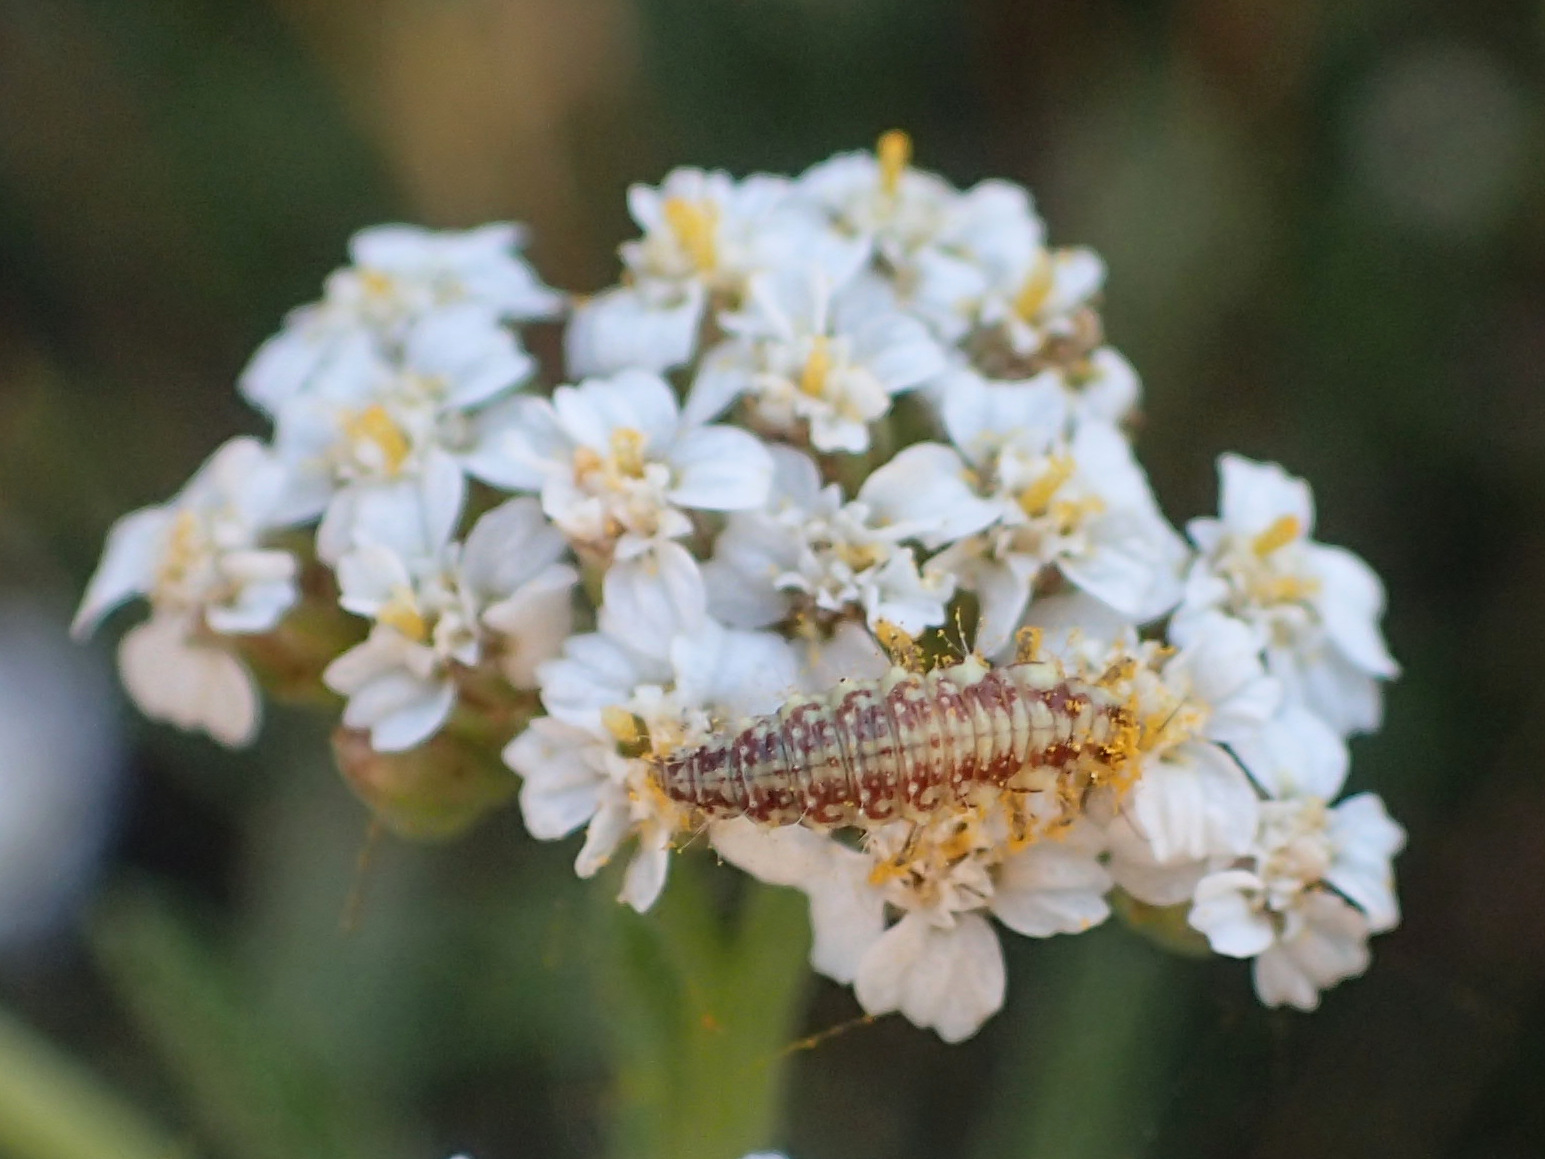
\includegraphics[width=\linewidth]{img/bogen/florfliegenlarve.jpg}
    \caption{Florfliegenlarve}
  \end{subfigure}
  \begin{subfigure}[b]{0.44\linewidth}
    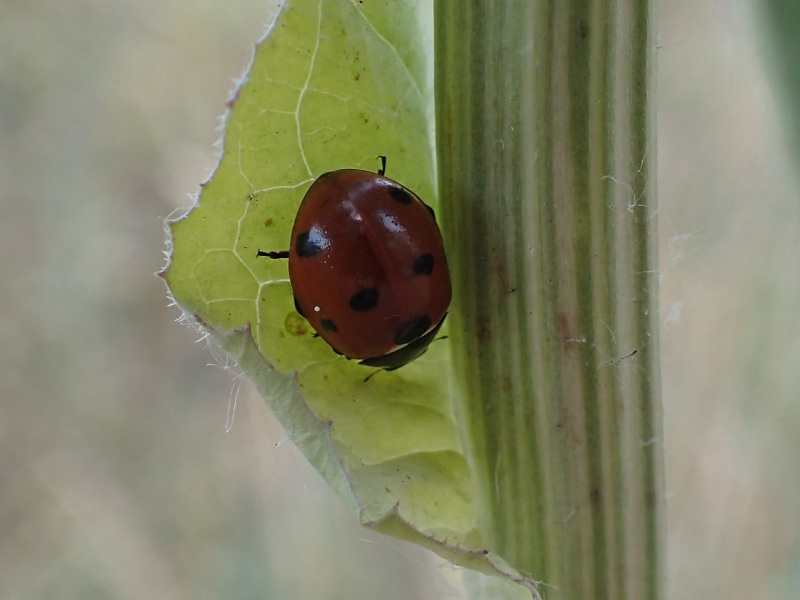
\includegraphics[width=\linewidth]{img/bogen/siebenpunkt.jpg}
    \caption{Siebenpunkt-Marienkäfer}
  \end{subfigure}
  \begin{subfigure}[b]{0.44\linewidth}
    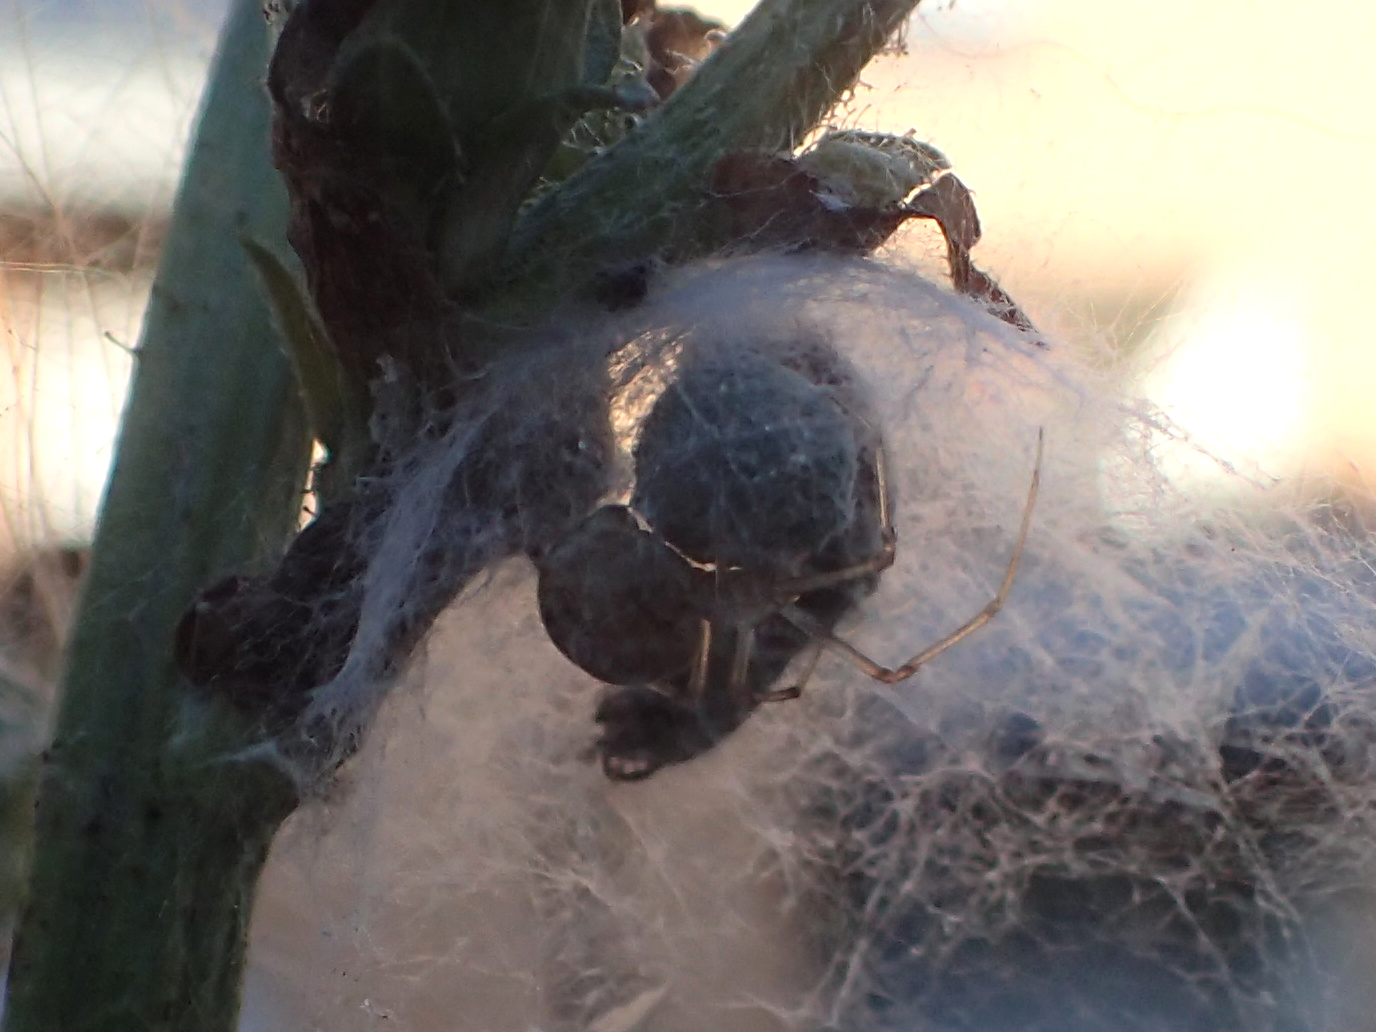
\includegraphics[width=\linewidth]{img/bogen/trapezspinne.jpg}
    \caption{Baldachinspinne}
  \end{subfigure}
  \caption{Insekten Hürther Bogen}
\end{figure}

Die Geldbinden-Furchenbiene ist eine Art warmer trockener Standorte, dies passt zum trockenen Standort der Blühfläche am Hürther Bogen.

\clearpage
\section{Berrenratherstr.}
\begin{figure}[h!]
  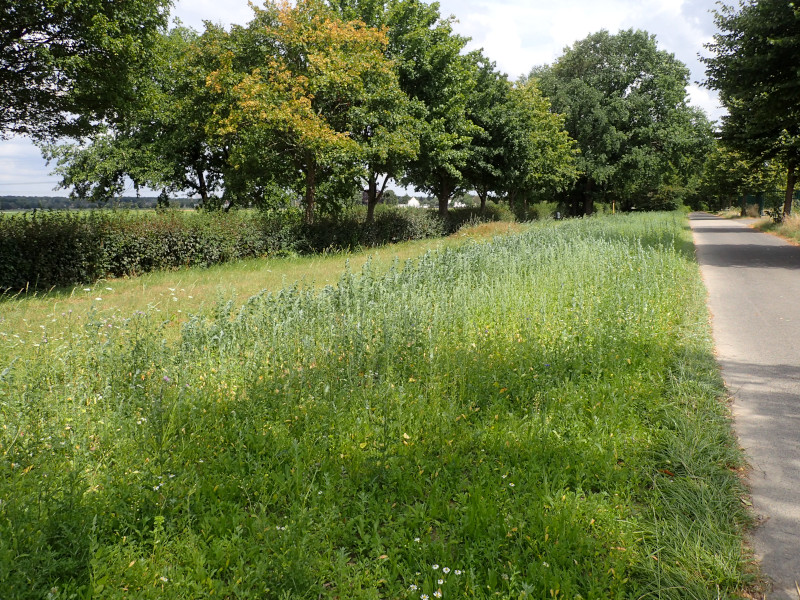
\includegraphics[width=\linewidth]{img/berrenrather/august.jpg}
  \caption{Berrenratherstr. 2. August 2020}
\end{figure}

Diese große Fläche bietet einiges an Potential, auch im Verbund mit den weiteren Blühflächen in der Nähe.

Durch die späte Aussaat im ersten Jahr war das Resultat noch nicht besonders überzeugend. Üblicherweise wird es im zweiten Jahr besser.

\clearpage
\section{Kendenich Friedhof}
\begin{figure}[h!]
  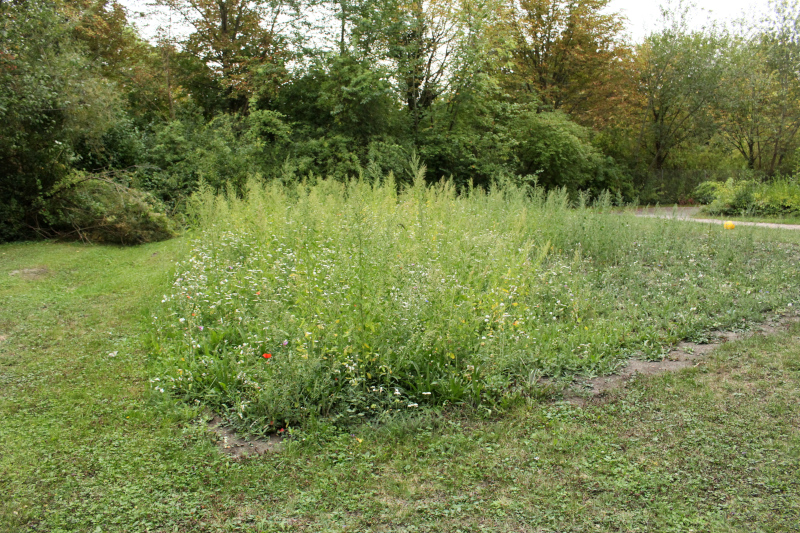
\includegraphics[width=\linewidth]{img/kendenich/september.jpg}
  \caption{Kendenich Friedhof. 4. September 2020}
\end{figure}

Von den neuen Flächen ist diese am besten angegegangen. Aber auch hier ist noch relativ viel Gänsefuß in der Fläche, der hoffentlich im nächsten Jahr weniger wird.

\clearpage
\section{Am Lintacker}
\begin{figure}[h!]
  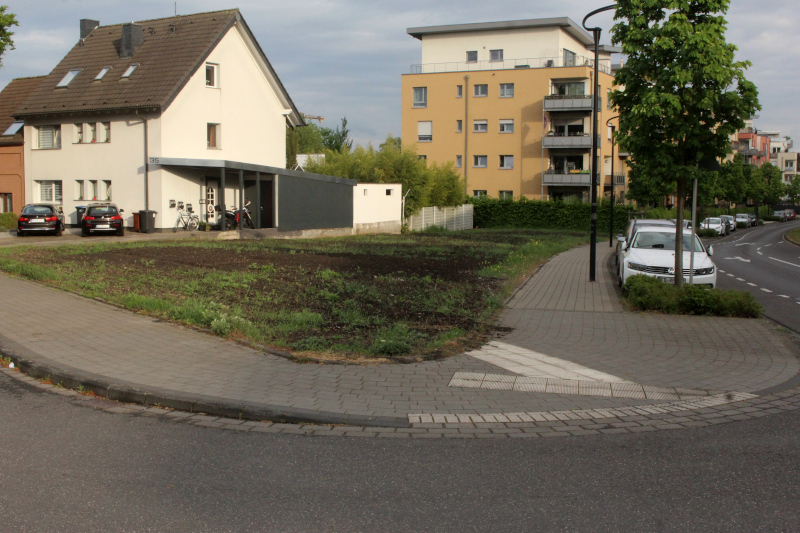
\includegraphics[width=\linewidth]{img/lintacker/april.jpg}
  \caption{Am Lintacker 28. April 2020}
\end{figure}

Hier wurde recht spät eingesät und wohl auch etwas zu tief. Daher dominierte hier der Gänsefuß.
Nächstes Jahr sollte es besser aussehen.

\clearpage
\section{De Bütt}
\begin{figure}[h!]
  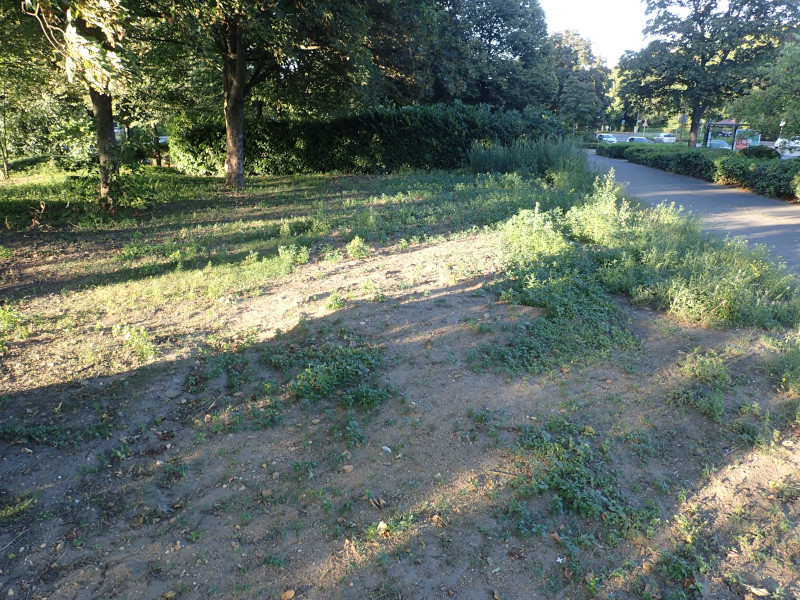
\includegraphics[width=\linewidth]{img/buett/juli.jpg}
  \caption{De Buett}
\end{figure}

Diese neu angelegte Fläche hat wegen einer Baumaßnahme nicht funktioniert.

Im nächsten Jahr sollten wir beobachten ob dort doch etwas überlebt hat, ggf. sollte hier nochmal eingesät werden.

\clearpage
\section{Aussicht}
Für 2021 werden wohl erstmal keine neuen Flächen angelegt werden, obwohl es noch potentielle Flächen gäbe.

Zunächst muss einmal mit allen Beteiligten geprüft werden, wie der Vorgehensweise und Pflege der Flächen funktioniert hat.

Mögliche Erweiterungen an den Flächen sollten jedoch besprochen werden, auch um die Mäharbeiten zu erleichtern.

Der BUND plant für 2021 einige Flächen per Handsense zu mähen, im Sinne einer schonenden, naturnahen und aktiven Pflege sowie weitere Kartierungen der Fauna und Flora auf und um die Blühflächen.

Die Webseite \href{https://hürth-blüht.de}{https://hürth-blüht.de} soll auch weiterhin gepflegt werden und über Neuigkeiten berichten.


\end{document}
